

\section{Plan}\label{plan}

\subsection{\texorpdfstring{Budget plan
}{Budget plan }}\label{budget-plan}

\begin{center}
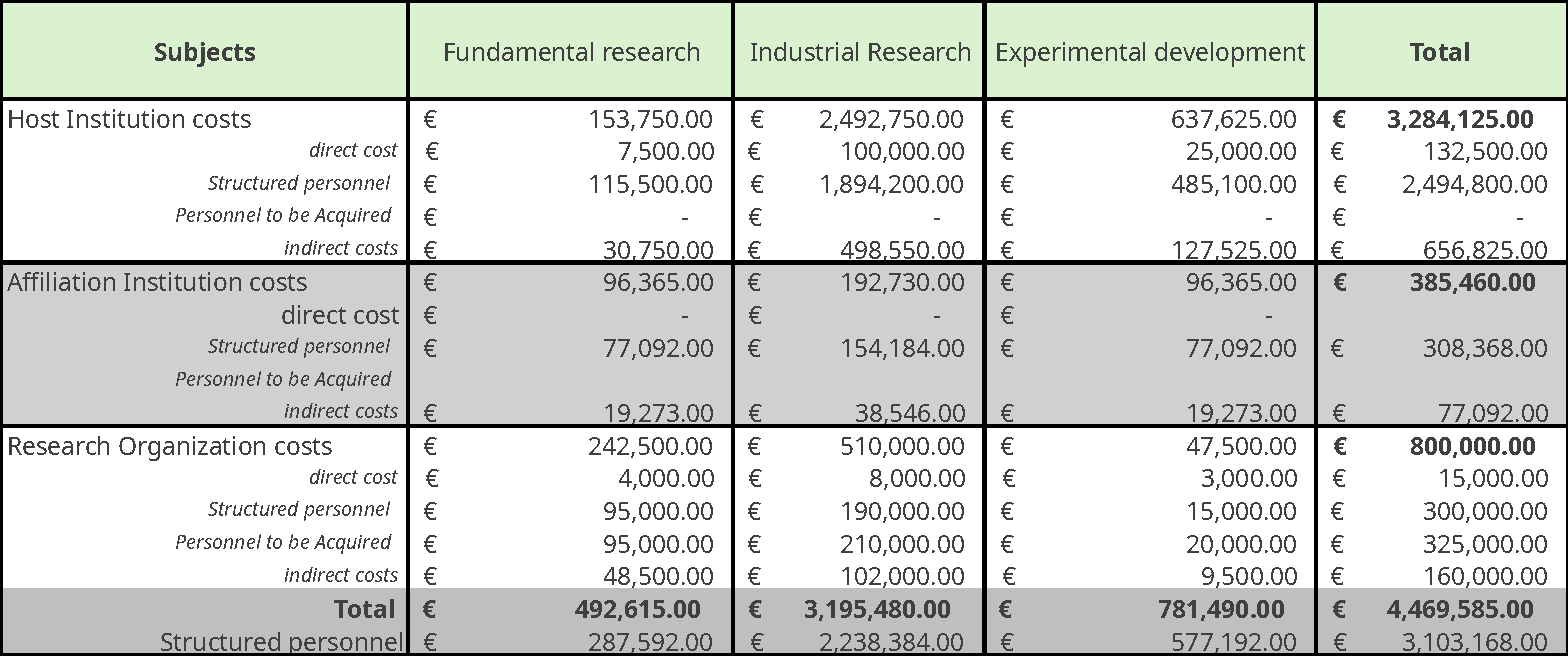
\includegraphics[width=\linewidth,height=0.78\textheight,keepaspectratio]{assets/image4.pdf}
\end{center}

\subsection{Co-financing aspects}\label{co-financing-aspects}

See \textbf{FISA\_2024\_00099\_Allegato B}

\subsection{\texorpdfstring{Time Schedule
}{Time Schedule }}\label{time-schedule}

\subsubsection{GANTT}\label{gantt}

Note:

\begin{itemize}
\item
  Each \textbf{Activity} will be documented following the continuous
  reporting approach. The document will report on the advancement and
  the results of the project itself.
\item
  If the activity generates a dataset, the consortium will evaluate if
  the dataset can be made publicly available.
\end{itemize}

The GANTT of the activities is reported in the Figure below.

\begin{center}
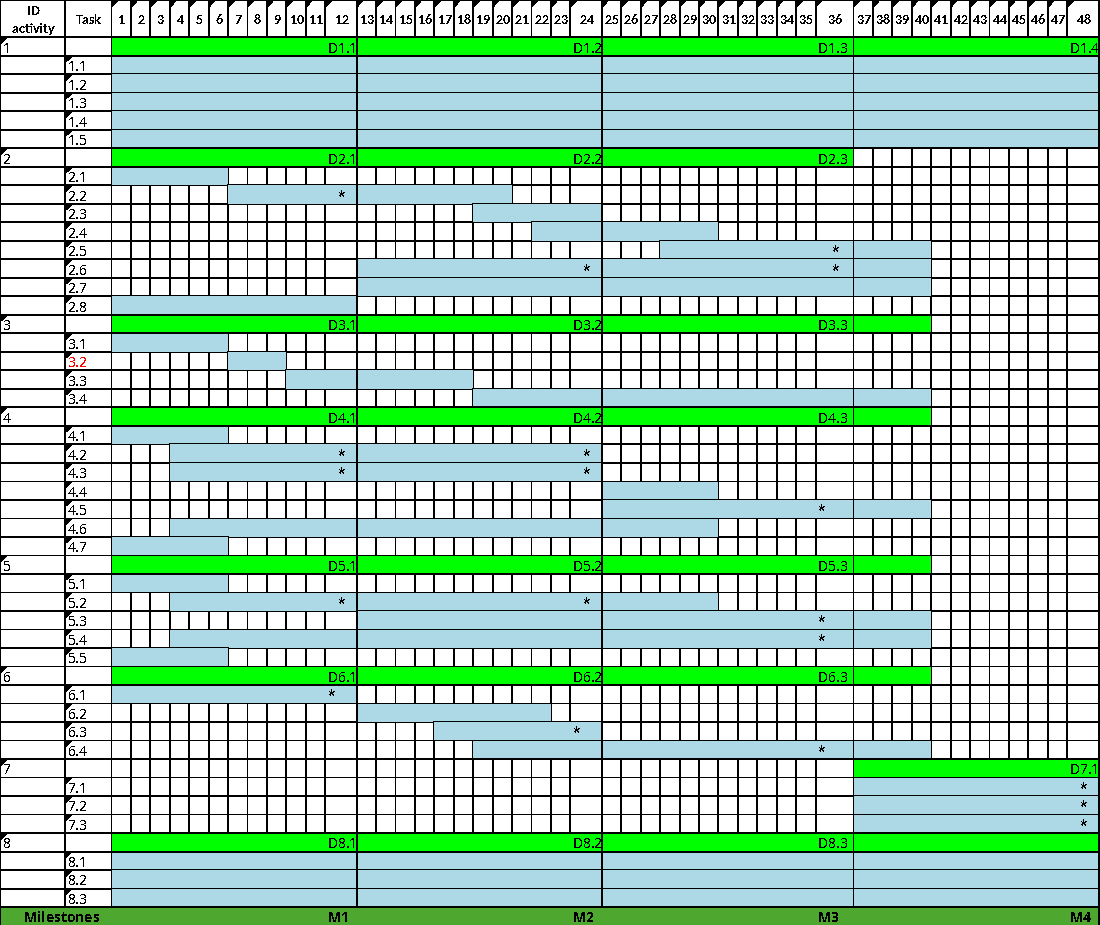
\includegraphics[width=\linewidth,height=0.72\textheight,keepaspectratio]{assets/image5.pdf}
\end{center}

\planfigurecaption{Figure 4 GANTT of the activities}

\subsubsection{List of Activities}\label{list-of-activities}

\begin{longtable}[]{@{}
  >{\raggedright\arraybackslash}p{(\columnwidth - 8\tabcolsep) * \real{0.1334}}
  >{\raggedright\arraybackslash}p{(\columnwidth - 8\tabcolsep) * \real{0.4789}}
  >{\raggedright\arraybackslash}p{(\columnwidth - 8\tabcolsep) * \real{0.2241}}
  >{\raggedright\arraybackslash}p{(\columnwidth - 8\tabcolsep) * \real{0.1627}}
  >{\raggedright\arraybackslash}p{(\columnwidth - 8\tabcolsep) * \real{0.0010}}@{}}
\toprule\noalign{}
\begin{minipage}[b]{\linewidth}\raggedright
\textbf{ID activity}
\end{minipage} & \begin{minipage}[b]{\linewidth}\raggedright
\textbf{Description}
\end{minipage} & \begin{minipage}[b]{\linewidth}\raggedright
\textbf{Start month}
\end{minipage} & \begin{minipage}[b]{\linewidth}\raggedright
\textbf{Duration}
\end{minipage} & \begin{minipage}[b]{\linewidth}\raggedright
\end{minipage} \\
\midrule\noalign{}
\endhead
\bottomrule\noalign{}
\endlastfoot
\textbf{1} & \textbf{Scientific, Technical, and Project Management} &
\textbf{1} & \textbf{48} & \\
\multicolumn{5}{@{}>{\raggedright\arraybackslash}p{(\columnwidth - 8\tabcolsep) * \real{1.0000} + 8\tabcolsep}@{}}{%
\textbf{Objectives:} The project Management will ensure that
\brand{Plan4ARI} contractual aspects are adhered to, including
technical, financial, administrative, and consortium coordination and
risk management, and will ensure that the project successfully achieves
its specified objectives on time and within budget. Coordination issues,
including contractual, legal, and administrative ones, are managed
within this work package. Furthermore, ensuring dependable contact with
the EU is an essential component of this WP over the
project\textquotesingle s duration.

\textbf{Task 1.1 General Management {[}\ul{CO FOUNDED ACTIVITY}{]}
M1-M48}

This task foresees setting up and maintaining project quality,
management procedures, reporting procedures, and templates for the
consortium. Administrative project management: legal representation of
the project, coordination, and development of implementation plans.
Follow-up and reporting of project progress. Project Meetings
coordination. Agreements preparation/maintenance. Setting up
communication guidelines, rules, forms, and templates and maintaining
internal communication levels and quality towards the financing
institution. To oversee the promotion of gender equality in the project
activities.

\textbf{Task 1.2 Financial management {[}\ul{CO FOUNDED ACTIVITY}{]}
M1-M48}

This task foresees setting up financial guidelines, reporting
procedures, and templates for consortium members, processing financial
statements, preparing audit certificates, and preparing detailed
financial plans.

\textbf{Task 1.3 Technical and Risk Coordination {[}\ul{CO-FOUNDED
ACTIVITY}{]} M1-M48}

This task foresees technical activities management and progress
follow-up. To ensure proper interaction between WPs. Intermediate
project results (deliverables) and project outputs quality monitoring.
To prepare and update the Data Management Plan. Manage technical risks
and decision-making during project execution---initial risks monitoring
and identifying new risks. Apply a contingency plan. Define and apply
corrective measures. All WP leaders will support CNR as members of the
Technical Committee.

\textbf{Task 1.4 Project Research Data Management {[}\ul{CO FOUNDED
ACTIVITY}{]} M1-M48}

Data will be collected as part of the project implementation only after
written informed consent of the enrolled subjects. Data will be fully
anonymized, with subjects identified only by numbers. Study participants
will be permitted to request removal of the coded data from the study
without penalty. The research will be conducted on ethical implications
according to the principles of widely recognized international texts and
codes of practice (e.g., the Helsinki Declaration). Project results will
fulfill the European GDPR and Data Protection Regulation superseding the
Data Protection Directive.

\textbf{Task 1.5 Creation of Advisory Board {[}\ul{CO FOUNDED
ACTIVITY}{]} M1-M48}

The Advisory Board will be set up in the first 6 Months of the project.
The board will be continuously updated on the project\textquotesingle s
progress and provide a technical audit of the deployed solutions to
balance the efficacy of the fundamental research with the exploitability
of the delivered solutions. The board will comprise Academic experts
external to the consortium and COMAU R\&D top-figures.} \\
\textbf{2}\phantomsection\label{activity-2} & \textbf{Low-code programming exploiting generative and
deliberative AI} & \textbf{1} & \textbf{36} & \\
% --- Revision A2 (23 September 2026): Activity 2 objectives and tasks -------
\activityrow{\revAii{%
\textbf{Objectives:} Activity 2 will develop a low-code programming
framework that enables process experts to configure robotic tasks
through natural-language requests. Generative AI will support
interpretation and knowledge extraction, while formal planners and
validators will produce and check executable plans. A capability and
skill registry will connect planning models to the actual robotic
system, using ROS2 interfaces, MI.RA/Dexter blocks, process
documentation and scene information. The modules will be integrated into
COMAU MI.RA/Dexter. The objectives remain a 66\% reduction in
programming time, programming by workers without prior
robotics-programming training, and management of three mobile
manipulators or four industrial robotic arms.}}
\activityrow{\revAii{%
\textbf{Task 2.1 Update of the scientific plan with the latest
state-of-the-art methodologies and tools {[}Fundamental Research{]}
M1-M12}

The task will review available generative and deliberative AI methods,
tools, performance, costs and integration requirements, and update the
scientific approach while maintaining the project objectives. D2.1 at
M12 will include both the updated scientific plan and the first running
mockup of the low-code module.

The mockup will follow the neuro-symbolic workflow described in
A2\_Research\_Project\_Proposal.pdf (9 July 2026, Section 2.1, Figure 1
and Section 3). Starting from an available PDDL domain, an operator
request and optional context, a graphical interface will support
structured JSON problem generation, deterministic PDDL compilation,
validation and repair, portfolio planning, and grounding of symbolic
actions to available ROS2/PlanSys2 executors. The initial demonstration
will address single-robot pick-and-place tasks. The delivery will
identify implemented functions and limitations and include versioned
artefacts, demonstration instructions, validation diagnostics, action
bindings and execution evidence.

A scientific manuscript presenting the mockup and its experimental
evaluation is planned for submission within one month of the present
revision, targeting 23 October 2026. IEEE Transactions on Automation
Science and Engineering (IEEE T-ASE) and IEEE Transactions on Industrial
Informatics (IEEE TII) are candidate venues; one of the two journals
will be selected. This is a dissemination target, separate from the M12
delivery, and does not imply acceptance or publication.}}
\activityrow{\revAii{%
\textbf{Task 2.2 PDDL Generation for Robotic Tasks with Lightweight LLMs
from Natural Language {[}Fundamental Research{]} M13-M24}

The task will extend the M12 mockup by investigating lightweight LLMs
for task interpretation, capability discovery, and planning model
generation. A typed intermediate representation will capture objects,
initial state, goals, constraints and unresolved information;
deterministic compilation and validator feedback will support PDDL
generation and bounded repair. A skill registry will associate
interfaces with parameters, preconditions, effects, resources and
provenance, combining runtime discovery with documentation and expert
verification. Research will progress from an available domain to domain
generation or adaptation from verified capabilities. Scene graphs will
provide structured facts and relations for assembly and disassembly
scenarios, using perception interfaces from the relevant activities.
Evaluation will compare direct generation with validated and
capability-grounded approaches.}}
\activityrow{\revAii{%
\textbf{Task 2.3 Validated Plan to Behaviour Tree Generation with
Time-Variance Modelling {[}Industrial Research{]} M18-M24}

This task will generate Behaviour Trees (BTs) from selected and
validated plans produced from the models developed in T2.2. It will
preserve action dependencies, resource constraints and execution
conditions, and bind BT action nodes to available skills. STN/STNU or
compatible temporal-network methods will support consistency checks,
dispatch and monitoring of uncertain durations. BehaviorTree.CPP and
PlanSys2/ROS2 will provide reference execution technologies. BT
generation belongs to T2.3 and does not replace symbolic planning. The
task will deliver the first time-variance-aware planner running in
MI.RA/Dexter for D2.2 at M24, through an initial adapter and execution
path developed with COMAU; T2.6 will consolidate industrial
integration.}}
\activityrow{\revAii{%
\textbf{Task 2.4 Task and Motion Planning Optimisation in a Digital Twin
Environment {[}Industrial Research{]} M22-M30}

The input comprises validated plans and the BT execution structures
generated in T2.3. The task will combine symbolic or temporal planning
with resource scheduling and motion-feasibility checks, according to the
application requirements. The digital twin will verify candidate
workflows, estimate durations and costs, and evaluate execution under
variability. MCTS will remain a research option for suitable stochastic
or online decision problems. Evaluation will measure feasibility,
makespan or cost, computational effort and solution quality against
defined solver baselines. Claims of optimality will state the model
assumptions and the evidence supporting them.}}
\activityrow{\revAii{%
\textbf{Task 2.5 Optimal Behaviour Tree Execution and Online Replanning
{[}Industrial Research{]} M28-M36}

The task will execute grounded BTs through the MI.RA/Dexter and
ROS2/PlanSys2 interfaces and monitor preconditions, expected effects,
scene state and timing. An anytime planning component will update
candidate plans during execution. Sudden changes will trigger bounded
repair, feasible heuristic replanning or an approved recovery behaviour.
Revised plans will pass the relevant validation and grounding checks
before dispatch. If no valid recovery is available within the execution
deadline, the system will stop the affected workflow and request
intervention. D2.3 at M36 will document task and motion planning with
online replanning, measured performance and remaining limitations.}}
\activityrow{\revAii{%
\textbf{Task 2.6 Integration of the Task Planning Framework inside
MI.RA/Dexter Low-Code {[}Industrial Research{]} M28-M36}

The task will consolidate and industrialise the initial MI.RA/Dexter
integration delivered with T2.3 at M24. It will map approved low-code
blocks and external skills to planning and execution interfaces, package
modules in containers, and address software dependencies, cybersecurity
and deployment requirements. Integration will preserve the boundary
between cognitive functions in the Open IPC and hard-real-time and
safety-critical control in the Core IPC. The code-generation service
described in the mockup may propose missing adapters or executors from
available interfaces; generated artefacts will require compilation,
testing and approval before deployment. Integration tests will verify
workflow execution, monitoring, recovery and rollback.}}
\activityrow{\revAii{%
\textbf{Task 2.7 Continuous Integration {[}Industrial Research{]}
M13-M36}

The task will maintain a shared development environment with version
control for software, models, prompts, schemas, skill registries and
benchmark cases. Automated checks will cover compilation, interface
compatibility, formal-model validation, plan-to-BT transformation,
action grounding and execution regressions. Release records will
identify dependencies, configurations, validation results and deployable
artefacts. The benchmark defined in T2.8 will be maintained and executed
throughout development, with technical evaluation contributed by
T2.2-T2.6 and end-user involvement coordinated with the Host
Institution.}}
\activityrow{\revAii{%
\textbf{Task 2.8 Benchmarking and Evaluation {[}Industrial Research{]}
M7-M12}

The task will define benchmark scenarios, ground truth, experimental
protocols and the baseline programming method by M12, and support
evaluation of the first running mockup. The protocol will preserve the
original coverage of 10 knowledge-base contexts and more than 100
contexts for each of PDDL generation, BT generation and task-planning
evaluation, with the definition and counting of contexts agreed by the
partners. Metrics will include problem and plan validity, repair
success, skill-grounding success, execution completion, plan quality,
latency and human intervention. Programming-time measurements will
distinguish cell setup, task programming and correction effort. The
initial mockup evaluation will use a defined subset; full KPI assessment
will continue through T2.2-T2.7 up to M36. The Host Institution will
involve operators and end-users in platform evaluation, preserving the
original programming-time and fleet-scale targets.}}
% --- end of Revision A2 block ---------------------------------------------
\textbf{3} & \textbf{Sensing for Context Awareness} & \textbf{1} &
\textbf{24} & \\
\multicolumn{5}{@{}>{\raggedright\arraybackslash}p{(\columnwidth - 8\tabcolsep) * \real{1.0000} + 8\tabcolsep}@{}}{%
\begin{minipage}[t]{\linewidth}\raggedright
\textbf{Objectives: Plan4ARI} will investigate using radar and 3D vision
sensors to monitor the robot\textquotesingle s working area,
investigating the sensor fusion of multiple sources to provide robust
operator tracking. The activity will be directly connected with the
results of activity 4 and 5. The modules developed in Activity 3 will be
integrated into MI.RA/Dexter COMAU framework.

\textbf{Task 3.1 Update of the scientific plan with the last
state-of-the-art methodologies and tools {[}Fundamental Research{]}
M1-M6}

AI tools and methods are rapidly growing in semantic segmentation and
pose estimation. A mandatory update of the scientific plan will be
performed at the start of the project, focusing on:

\begin{itemize}
\item
  The state of the art of the available tools, their costs, and
  performance
\item
  The state of the art of academic methodologies. If notable
  improvements emerge that may surpass the planned approach, adjustments
  to the technical approach will be made to maintain project objectives.
\end{itemize}

\textbf{Task 3.2 Radar sensor integration for scene monitoring
{[}Industrial Research{]} M7-M9}

In the market, radar technologies have started to offer the option of
having 3D point clouds of objects inside the scene.

The task will perform a detailed market investigation, and the more
promising sensors will be acquired and tested.

The sensor acquisition will then be packed inside a set of libraries
that can be easily interfaced with the ROS2 network of devices.

\textbf{Task 3.3 Fusion of radar sensor data and camera data
{[}Industrial Research{]} M10-M16}

The challenge consists of fusing data from different sensors that are
updated at different frequencies. This issue has been investigated
mainly in automotive to ensure safe driving. The most common approach
uses robust multi-object detection and tracking methods for moving
objects. First, the radar and camera perform target detection
independently, and the detection results are correlated in the image
plane to generate a random finite set with an object type. Then, based
on the Gaussian mixture probability hypothesis density (GM-PHD)
algorithm framework, the tracking process will be refined through
elliptic discriminant thresholds, an attenuation function, and
simplified pruning methods. The module will be integrated as a
functional block inside the MI.RA/Dexter Platform.

\textbf{Task 3.4 Semantic Segmentation {[}Industrial Research{]}
M17-M24}

The state-of-the-art semantic segmentation of images for identifying the
Cartesian pose of objects involves several advanced techniques, mainly
combining deep learning for segmentation and pose estimation approaches.
MI.RA/Dexter already provides a few modules for pose estimation, and the
host institution will put significant effort into bringing such modules
to dramatically better performance.

Deep Learning for Semantic Segmentation is often used for the
segmentation, and modern systems utilize mainly Convolutional Neural
Networks (CNNs) and Transformers to perform pixel-wise classification of
images. Some key methods and architectures include Fully Convolutional
Networks (FCNs), U-Net, DeepLab (v3+), and Mask R-CNN.

Concerning 3D Object Pose Estimation, the task is generally tackled
using Keypoint Detection Methods (like PoseCNN), or 6D Pose Estimation
(like PVNet and PoseRBPF).

The recent trends and techniques are mainly focused on the adoption of
Transformers for Segmentation and

End-to-End Pose Estimation Models. Methods such as ``PoseNet'' and
``Single-shot pose estimation networks (SSD-6D)'' allow simultaneous
object detection, segmentation, and pose prediction in one unified
framework. Also, ``Graph Neural Networks (GNNs)'' are extremely
promising.

The task will set up a benchmarking environment for testing the most
promising state-of-the-art methods. The dataset will be created by
selecting the most common requests from the COMAU users.

The highest-performing algorithm will be added to the MI.RA/Dexter
platform.
\end{minipage}} \\
\textbf{4} & \textbf{Local and Global Autonomous Motion Planning} &
\textbf{1} & \textbf{36} & \\
\multicolumn{5}{@{}>{\raggedright\arraybackslash}p{(\columnwidth - 8\tabcolsep) * \real{1.0000} + 8\tabcolsep}@{}}{%
\begin{minipage}[t]{\linewidth}\raggedright
\textbf{Objectives: a} key aspect of modern collaborative robotic
application is advanced motion planning. \brand{Plan4ARI} aims to
develop and deploy motion planners able to plan trajectories for a team
of manipulators, in a collaborative dynamic environment. The modules
will be integrated in the MI.RA/Dexter COMAU framework.

\textbf{Task 4.1 Update of the Scientific Plan with the latest
State-of-the-Art Methodologies and Tools for Motion Planning
{[}Fundamental Research{]} M1-M6}

\begin{itemize}
\item
  Motion planning in robotics has seen rapid advancements, especially in
  real-time adaptability and high-dimensional search efficiency. This
  task will analyze the latest algorithms and frameworks, including
  their performance, computational demands, and scalability.
\end{itemize}

\textbf{Task 4.2 Informed Sample-Based Optimal Motion Planning for teams
of mobile manipulators in dynamic environments {[}Industrial Research{]}
M4-M24}

The task deals with two goals.

\begin{itemize}
\item
  It aims to create a mixed sampling strategy combining global and local
  informed sampling for asymptotically optimal sampling-based path
  planners. Local informed sampling oversamples the neighborhood of the
  current solution to quickly reach a local optimum, while globally,
  informed sampling guarantees asymptotic optimality.
\item
  We propose an asymptotically optimal algorithm using the mixed
  sampling strategy and dynamically adjust the trade-off between global
  and local sampling. We expect this approach to outperform
  state-of-the-art planners, such as Informed-RRT∗, on different class
  problems. The methodology will then be integrated into an anytime
  planning framework to quickly provide a suitable solution in complex,
  high-dimensional search spaces. The core idea consists of building a
  graph that connects paths to the same goal, allowing the exploitation
  of pre-calculated paths. When an obstacle blocks the current path, it
  looks for a new one by trying to connect the current path to the other
  available ones. If a connection is found, it can search for better
  solutions during the remaining time.
\end{itemize}

\textbf{Task 4.3 Model Predictive Control for Optimal Adaptive
Micro-interpolation {[}Industrial Research{]} M4-M24}

The robot micro-interpolator running on the Core IPC (Figure 1) will
exploit an MPC methodology. The MPC has the property of being able to
predict \textbf{future states in a predefined time window.} In other
words, it is possible to continuously create a queue of references for
the low-level control with the dimension of the time window. MPC uses a
dynamic model of the robot to predict its future states (e.g.,
positions, velocities, and accelerations) over a finite time horizon.
This allows it to generate smooth and feasible trajectories for the
robot to follow. Indeed, the MPC can \textbf{handle Constraints.}
Industrial robotics usually has constraints on joint limits, velocity,
acceleration, and even workspace boundaries. MPC can naturally
incorporate these constraints into the optimization process, ensuring
that the generated trajectory respects these physical limits. The
resulting trajectory will be optimal for the selected cost function
(typically including terms for trajectory tracking error, energy
consumption, and smoothness). This ensures that the robot follows the
desired trajectory as accurately and efficiently as possible.

Modern advancements in computational power and optimization algorithms
make it feasible to implement MPC in real-time, even for high-speed
robotic systems. MPC can continuously update the control actions based
on real-time feedback, making it robust against disturbances and model
inaccuracies.

The MPC will allow an easy and effective interface with the sensor for
visual servoing while offering both Cartesian and joint interfaces. The
MPC will be designed by exploiting the tools offered by COMAU to
virtualize the robot.

\textbf{Task 4.4 Integration of the Motion Planning Framework inside
MI.RA/Dexter low-code {[}Industrial Research{]} M25-M30}

Integrating the motion planning pipeline inside the COMAU low-code
programming tools will allow a straightforward digital twin of the
setup. MI.RA/Dexter allows the creation of ``dockerized'' actions. This
means that it is possible to integrate external code by creating a
container and wrapping it through proper interfaces.

This modular approach allows code integration in a network of
computation units.

The deployment of the task planning module will follow a two steps
approach:

\begin{itemize}
\item
  Analysis of the SW modules, dependencies, and security constraints
\item
  Deployment of the proper actions to embed the code in the platform.
\end{itemize}

The code embedding will be done eventually, reusing the code already
deployed by the research organization. When the industrial requirements
of such code are not met, the code will be re-engineered to grant
maximum safety to the full setup.

\textbf{Task 4.5 Integration of the MPC trajectory micro-interpolator
inside the COMAU Core IPC {[}Deployment{]} M31-M36}

Integrating the MPC inside the COMAU Core IPC will be a technicality
that will require strong teamwork between COMAU and the Research
Organization teams. The need for the module to support both a
low-frequency async communication channel towards the external world and
a hard-real real-time communication channel towards the robot will
introduce a complex SW architecture. In addition, the MPC should also
offer an interface for synchronous input communication. The MPC will
mainly be designed to safely change the speed override of the robot
according to its working condition.

\textbf{Task 4.6 Continuous Integration {[}Industrial Research{]}
M4-M36}

The SW development will follow a continuous integration paradigm. A
cloud will be available to share the code among all the teams. Proper
mechanisms for the versioning and remote checking will be implemented.
The SW will provide functional tests, and the SW development will be
tracked according to the gold rules for SW deployment.

\textbf{Task 4.7 Benchmarking and Evaluation {[}Industrial Research{]}
M1-M6}

An extensive set of application examples will be defined in the first
six months of the activity. The researchers will have the application
goals as north-star to direct the deployment of the SW. The partners
will agree upon the design of the experiments. The Host Institution will
evaluate the performance by inviting operators and end-users to test the
platform.
\end{minipage}} \\
\textbf{5} & \textbf{Neural Robust Motion Control} & \textbf{1} &
\textbf{36} & \\
\multicolumn{5}{@{}>{\raggedright\arraybackslash}p{(\columnwidth - 8\tabcolsep) * \real{1.0000} + 8\tabcolsep}@{}}{%
\begin{minipage}[t]{\linewidth}\raggedright
\textbf{Objectives:} Neural control algorithms constitute a frontier for
robotic control but with a limited number of applications.
\brand{Plan4ARI} aims to investigate and integrate the last neural
control algorithms for robot low-level control going beyond the current
industrial SOTA. The modules developed will be integrated into
MI.RA/Dexter COMAU framework.

\textbf{Task 5.1 Update of the scientific plan with the last
state-of-the-art methodologies and tools {[}Fundamental Research{]}
M1-M6}

AI tools and methods are rapidly growing in semantic segmentation and
pose estimation. A mandatory update of the scientific plan will be
performed at the start of the project. The update will focus on:

\begin{itemize}
\item
  The state of the art of the available tools, their costs, and
  performance
\item
  The state of the art of academic methodologies. The advancement could
  be overcome by the proposed approach in the next year. In such a case,
  the technical approach will also be updated, maintaining the same
  objectives.
\end{itemize}

\textbf{Task 5.2 Design of the neural controller with prescribed
performance constraint architecture {[}Industrial Research{]} M4-M30}

As discussed in the dedicated section, the team will conceive and
implement a neural controller with the prescribed performance constraint
architecture. The implementation of such a control law will follow the
standard design procedures:

\begin{itemize}
\item
  The mathematical model considering the lumped-elastic effect will be
  investigated and deployed
\item
  The control law will be designed, and the stability will be proven
\item
  The test will be primarily done using ad-hoc simulators in MATLAB,
  exploiting the wide framework developed in COMAU in the last 30 years.
\end{itemize}

Once the control is confirmed and delivered, its implementation in C++
will be performed. First, the implementation will move small mechanisms
controlled by a ROS2 architecture. The implementation in the COMAU
controller will be in the following task.

\textbf{Task 5.3 Integration of the Motion Planning Framework inside the
Open IPC {[}Industrial Research{]} M12-M36}

Integrating the motion controller inside the COMAU Open IPC will allow a
straightforward digital twin to be set up. MI.RA/Dexter allows the
creation of ``dockerized'' actions. This means that it is possible to
integrate external code by creating a container and wrapping it through
proper interfaces.

This modular approach allows code integration in a network of
computation units.

The deployment of the task planning module will follow a two steps
approach:

\begin{itemize}
\item
  Analysis of the SW modules, dependencies, and security constraints
\item
  Deployment of the proper actions to embed the code in the platform.
\end{itemize}

The code embedding will be done eventually, reusing the code already
deployed by the research organization. When the industrial requirements
of such code are not met, the code will be re-engineered to grant
maximum safety to the full setup.

\textbf{Task 5.4 Continuous Integration {[}Industrial Research{]}
M4-M36}

The SW development will follow a continuous integration paradigm. A
cloud will be available to share the code among all the teams. Proper
mechanisms for the versioning and remote checking will be implemented.
The SW will provide functional tests, and the SW development will be
tracked according to the gold rules for SW deployment.

\textbf{Task 5.5 Benchmarking and Evaluation {[}Industrial Research{]}
M1-M6}

An extensive set of application examples will be defined in the first
six months of the activity. The researchers will have the application
goals as north-star to direct the deployment of the SW. The partners
will agree upon the design of the experiments. The Host Institution will
evaluate the performance by inviting operators and end-users to test the
platform.
\end{minipage}} \\
\textbf{6} & \textbf{Human-Robot Trustiness Evaluation and Assessment} &
\textbf{7} & \textbf{36} & \\
\multicolumn{5}{@{}>{\raggedright\arraybackslash}p{(\columnwidth - 8\tabcolsep) * \real{1.0000} + 8\tabcolsep}@{}}{%
\textbf{Objectives:} \brand{Plan4ARI} develops a tool to support
manufacturers in assessing the workers\textquotesingle{} engagement when
working with an AI-powered collaborative robot.

\textbf{T6.1 Subjective Evaluation: Design of the Questionnaire
{[}Industrial Research{]} M7-M9}

The goal is to investigate trust in a workstation, feelings, perceptions
of the relationship between robot and operator, and other information.
The following points are of interest: i) Scholarship/skills (attended
classes about the workstation, about cobot, safety included); ii) Trust
in the safety of the workstation, i.e., trust of being not physically
damaged by the motion of the cobot while collaborating with it; iii)
trust in software for safety installed on cobot; iv) trust that
workstation as cobot and operator effectively accomplishes the job; v)
degree of relevance attributed to the fact that the machine is a cobot
instead of ``any other'' machine; vi) degree of feeling cobot as just a
tool or as something close to colleague concepts; vii) degree of feeling
playing a role that is active/leading/equal to cobot or being driven
by/subject to cobot; viii) mental/physical stress before, during and
after shifts with cobot; ix) impressions after a shift. Such topics have
been drafted considering the manufacturing scenario. Debating with
operators will be included to define topics. Each topic is expected to
lead to one or more questions/scale items.

\textbf{T6.2 Subjective Evaluation: Questionnaire Validation
{[}Industrial Research{]} M10-M16}

We will exploit their contact at the national and international levels
to contact companies to reach out to at least \hl{50} workers who will
be asked to complete the evaluation form. An online tool will be
prepared. CNR will coordinate the scientific part, analyze the data,
proceed with the interview as needed, and manage the GDPR-related
aspects.

\textbf{T6.3 Subjective Evaluation: Questionnaire Deployment
{[}Industrial Research{]} M17-M24}

According to the dataset acquired in Task 6.2, a statistical evaluation
will be performed to identify the statistically robust items coherent
with the target scenario. The final evaluation form will be deployed
according to the number of people evaluated in Task 6.2.

\textbf{T6.4 Subjective Evaluation: Evaluation Campaign, dataset
creation synthesis {[}Industrial Research{]} M24-M36}

The final campaign will follow the approach in Task 6.2. The target
consists of having +\hl{100} workers interviewed.} \\
\textbf{7} & \textbf{Targeted Demonstrator} & \textbf{36} & \textbf{48}
& \\
\multicolumn{4}{@{}>{\raggedright\arraybackslash}p{(\columnwidth - 8\tabcolsep) * \real{0.9990} + 6\tabcolsep}}{%
\begin{minipage}[t]{\linewidth}\raggedright
\textbf{Objectives:} the goal of this activity is to demonstrate all the
\brand{Plan4ARI} technologies on a targeted demonstrator provided by
COMAU. The projects will demonstrate technologies on three different
demonstrators coming from different industrial sectors. All the three
demonstrators will exploit the technologies developed in the project.

\textbf{Task 7.1 Picking random objects from a warehouse
{[}Deployment{]} M36-M48}

The use case includes the manipulation of a huge variety of objects in a
warehouse.

With the massive spread of the e-commerce the request for automatic
applications in warehouses is increasing. The application requires the
manipulation of objects of a completely different nature, such as soft
objects, clothes, or without standardized packaging.

Currently this activity is mainly manual, imposing with high production
rate and repetitive tasks, causing high stress on operators. The working
environment is extremely dynamics and doesn't allow the installation of
fences or rigid layout. The application involves the use of industrial
mobile manipulator to pick a certain object from position A and release
the object in a position B.

The operator will teach the possible objects to be found to the robot.

The operator will teach the task to the robot with natural language,
such as ``hey robot! Pick the red t-shirt in box A and then put the
t-shirt in box B''.

The system will interpret the command and translate the instruction into
the robot program.

A task planner will schedule the tasks to all the manipulators necessary
to reach the goal.

The motion planner will plan the trajectories for all the manipulators
involved in the task avoiding the known object in the scene. A network
of sensors continuously monitors the scene tracking the presence of the
operator. In case of possible collision, the motion planner will replan
the trajectory to avoid any possible collision. The operators involved
in the demonstration will be asked to answer the questionnaire developed
in activity 6.

The challenges in such a scenario are:

\begin{itemize}
\item
  The easiness in the KB creation
\item
  The robot accurate localization
\item
  The accurate semantic segmentation and pose estimation
\item
  The offline motion planning
\item
  The online motion planning -- if the human is present
\end{itemize}

\textbf{Task 7.2 Remanufacturing of mechanical components
{[}Deployment{]} M36-M48}

Remanufacturing of components and devices is becoming a key aspect for
making more sustainable the manufacturing sector. Remanufacturing avoids
waste production and reduces the request of raw materials. The use case
will involve the remanufacturing of a mechanical device. The type of
device will be decided during the project. The use case scenario
involves a non-robotic expert which will guide the robot through natural
commands such as ``Hey robot! Remove cover A from the device using the
tool C and B''.

The system will automatically generate robot instructions involving the
task and motion planner generating an optimal task sequence and optimal
trajectories.

Each task could require different control targets:

\begin{itemize}
\item
  Force/Admittance setpoint in interaction tasks
\item
  High performance in Cartesian Error Tracking
\item
  \ldots{}
\end{itemize}

Thanks to the low-level neural controllers, and the advanced dynamics
modelling, the robot interaction with the environment during the
disassembly tasks will be handled with higher performance compared to
the current standard for industrial robot controllers, i.e. low-level
control developed in \brand{Plan4ARI} will guarantee an extremely high
precision in robot-environment interaction forces estimation, such as
during parts separation, or during the machining of components.

The operator will be fully involved in the process of being free to
enter and intervene in the robot working area.

The tracking system made by the network of sensors will continuously
track the operator. In case the operator enters the robot working area
the motion planner will replan the robot trajectories to avoid any
possible collision. In case the trajectory replanning will not be
possible, the task planner will dynamically reschedule the task sequence
allocating the robot to a different task. This iterative interaction
will continue until the remanufacturing task is ended. The operators
involved in the demonstration will be asked to answer the questionnaires
from activity 6.

The challenges in such a scenario are:

\begin{itemize}
\item
  The easiness in the KB creation
\item
  The robot accurate localization
\item
  The accurate semantic segmentation and pose estimation
\item
  The sensor fusion to achieve safety and performance in localization
\item
  The online motion planning
\item
  The hard-real time motion planning (MPC) to avoid any issue
\item
  The performance of the low-level control
\item
  The users' acceptance level for the AI-powered robot
\end{itemize}

\textbf{Task 7.3 Welding of plates in huge boat {[}Deployment{]}
M36-M48}

The production of cargo and cruise boats deeply requires the use of
welding processes to join huge plates. The welding process is currently
done manually directly onsite (i.e. on the boat). The working conditions
are severe, exposing the workers to unsafe and unhealthy working
environments. The high demand of manual labor is also pushing the naval
production to countries with a lower cost of manpower. For these reasons
automation and robotics can bring innovation to the sector. Many
barriers are anyway present in this working environment, such the
extremely complex, dynamic and cluttered environment which constitutes
the production site of a huge boat. Obviously, given the huge dimensions
of the boat, the welding robot will be a welding mobile manipulator. The
use of fences will not be possible since welding mobile manipulator will
move around the boat where it is required to do the task. As for the
other use cases, even in this case all the modules developed in
\brand{Plan4ARI} will be extensively used. An operator, expert about
the welding process, but not of robotics programming, will guide the
robot through voice commands, indicating which plates need to be welded.
As for the other use cases, the control stack will generate optimal
trajectories avoiding known obstacles. At the same time, the working
area will be monitored by the network of sensors, in case of operator
approaching to the manipulator during the task execution, the replanning
will be avoided, since welding is a process which do not allow to
deviate from the nominal path. The process will only be safely stopped
and resumed once the operator will be outside from the dangerous area.
The operators involved in the demonstration will be asked to answer the
questionnaire developed in activity 6.

The challenges in such a scenario are:

\begin{itemize}
\item
  The easiness in the KB creation
\item
  The robot accurate localization
\item
  The accurate semantic segmentation and pose estimation
\item
  The sensor fusion to achieve safety and performance in localization
\item
  The online motion planning
\item
  The hard-real time motion planning (MPC) to avoid any issue
\item
  The performance of the low-level control
\item
  The users' acceptance level for the AI-powered robot
\end{itemize}
\end{minipage}} & \\
\textbf{8} & \textbf{Communication and Dissemination} & \textbf{1} &
\textbf{48} & \\
\multicolumn{5}{@{}>{\raggedright\arraybackslash}p{(\columnwidth - 8\tabcolsep) * \real{1.0000} + 8\tabcolsep}@{}}{%
\textbf{Objectives:} (i) To continuously communicate the project
activities and adequately disseminate results linked to the project
exploitation plans. (ii) To conduct a proper market analysis and
consequent management of project exploitable results supported by
business case methodologies. (iii) To manage the exploitation plan,
considering business plans, decisions, and agreements backed by
protected IPR and suitable business models.

\textbf{Task 8.1 Communication activities M1-M48}

This task will provide channels to communicate project objectives,
status, progress, and results to the public. Essential elements of
project communication are the project website, which is to be launched
in M1 and updated throughout the project with news, information, and
public deliverables produced by the project. Public Communication
Materials -- consisting of press releases, a project presentation, a
digital project poster, a brochure to be adapted/printed on demand, and
project videos related to project concepts and use case demonstrators.
News and posts on digital media -- the publication of news and posts
will be planned and reported regularly.

\textbf{Task 8.2 Dissemination activities M1-M48}

This task concerns disseminating project objectives, scientific
relevance, and exploitable applications; detailed results will be
planned. Dissemination actions that will be considered are Workshops,
Seminars, Scientific publications, and primarily in charge of academic
research institutions. Industries and tech providers will conduct trade
fairs and exhibitions. All partners will contribute to the definition of
the dissemination activities.

\textbf{Task 8.3 Market analysis and Exploitation plan M1-M48}

This task will establish and maintain an exploitation culture throughout
the project. This will be done through systematic exploitation
activities during the project, accelerating the market adoption of
project results. Critical elements of exploitation activities are cost
and market analysis, which assesses the market potential and impact of
project results tailored to partner exploitation channels. This analysis
includes business modeling and potential future capital requirements
associated with scaling up. Identification of Exploitable results, a
project exploitable results table to identify, synchronize, and conduct
efficient planning and management of the project foreground. Actions
will be identified to develop and execute exploitation activities
associated with each result, and management of the collective project
foreground will be a part of periodic reporting and project meetings. An
Exploration plan includes a study of the exploitation potential of each
project result and the exploitation strategy, as well as establishing an
appropriate calendar. Patent surveys and filing ongoing patent
surveillance studies will allow for correctly managing the
project\textquotesingle s patentable results. Potential patents will be
managed following the roles and priorities of the Exploitation
Agreement.} \\
\end{longtable}

\subsubsection{\texorpdfstring{List of Deliverables
}{List of Deliverables }}\label{list-of-deliverables}

\begin{itemize}
\item
  D1.1 Management Report, M12
\item
  D1.2 Management Report, M24
\item
  D1.3 Management Report, M36
\item
  D1.4 Management Report, M48
\item
  D2.1 Scientific Plan and First Running Mockup of the Low-Coding
  Module, M12
\item
  D2.2 First Running Time-Variance Aware Planner Running in MI.RA/Dexter
  Environment, M24
\item
  D2.3 Optimal Task and Motion Planning with online replanning module,
  M36
\item
  D3.1 Scientific Plan and First Running Mockup for the sensing module,
  M12
\item
  D3.2 Sensing Methodologies and First Prototypes Release, M24
\item
  D3.3 Sensing Modules integrated in the COMAU IPC, M36
\item
  D4.1 Scientific Plan and First Mockup of the Motion Planning Modules,
  M12
\item
  D4.2 Motion Planners Modules Prototypes, M24
\item
  D4.3 Motion Planners Modules Prototypes integrated in the COMAU IPC,
  M36
\item
  D5.1 Scientific Plan and First Mockup of the Neural Control
  Architecture, M12
\item
  D5.2 First Release of the Neural Controller Prototype, M24
\item
  D5.2 Neural Control Architecture integrated in the COMAU IPC, M36
\item
  D6.1 Scientific Plan and First Questionnaire Release, M12
\item
  D6.2 Second Questionnaire Release, M24
\item
  D6.3 Campaign Evaluation Report, M36
\item
  D7.1 Demonstrators
\item
  D8.1 Exploitation, Communication, Dissemination Report, M12
\item
  D8.2 Exploitation, Communication, Dissemination Report, M24
\item
  D8.3 Exploitation, Communication, Dissemination Report, M36
\end{itemize}

\subsubsection{List of Milestones}\label{list-of-milestones}

\begin{itemize}
\item
  Milestone 1, M12 (Mean of verification: D1.1, D2.1, D3.1, D4.1, D5.1,
  D6.1, D7.1, D8.1)
\item
  Milestone 2, M24 (Mean of verification: D1.2, \revAii{D2.2}, D3.2, D4.2, D5.2,
  D6.1, D7.2, D8.2)
\item
  Milestone 3, M36 (Mean of verification: D1.3, D2.1, D3.3, D4.3, D5.3,
  D6.1, D7.3, D8.3)
\item
  Milestone 4, M48 (Mean of verification: D1.4, \revAii{D2.3}, D3.4, D4.4, D5.4,
  D6.1, D7.4, D8.4)
\end{itemize}

\begin{quote}
The Scientific Coordinator
\end{quote}

\begin{center}

\includegraphics[width=0.42\linewidth,height=0.78\textheight,keepaspectratio]{assets/image6.png}
\end{center}
